\section{Questions and Answers}
\label{sec:questions}

\subsection{Question 1}
\label{subsec:q1}
\textbf{Which of the following metrics is the correct one to evaluate LLaMA~3 intrinsically
in the next-token-prediction task?}

\begin{itemize}
    \item F1 Score
    \item BLEU
    \item \answer{Perplexity}
    \item Accuracy
\end{itemize}

\answer{Perplexity is the standard metric for language modeling tasks (i.e., next token prediction).
It measures how “surprised” the model is by the real sequence.}

\subsection{Question 2}
\label{subsec:q2}
\textbf{What is the difference between Cross-Attention and Causal Attention?}

\answer{\textit{Causal attention} is an attention mechanism that involves a single sequence,
where each token has access to the previous tokens, but not the future ones.
It is common in autoregressive models like GPT and is used for text generation.
\textit{Cross-Attention} is another attention mechanism that involves two sequences: a source
and a target (typically the encoder and decoder in a seq2seq model).
In this case, the target sequence has access not only to its own generated tokens, but also
the tokens from the source sequence - representing a "crossing'' of information between the two.
It is used in translation and text summarization tasks.}

\subsection{Question 3}
\label{subsec:q3}
\textbf{Which of the following Preference Optimization algorithms requires a dedicated
    (or separate) reward model?}

\begin{itemize}
    \item Direct Preference Optimization
    \item \answer{Proximal Preference Optimization (PPO)}
\end{itemize}

\answer{Inspired by Proximal Policy Optimization, PPO requires training a separate reward model
to guide the main policy.}


\subsection{Question 4}
\label{subsec:q4}
\textbf{Which of the following generation techniques randomly samples one word at each step?
Mark all that apply.}

\begin{itemize}
    \item Greedy Decoding
    \item \answer{Nucleus Sampling}
    \item \answer{Top-K Decoding}
    \item Beam Search
\end{itemize}

\answer{Both use sampling (top-p or restricting to top-k most probable tokens). Greedy Decoding
and Beam Search do not introduce randomness.}

\subsection{Question 5}
\label{subsec:q5}
\textbf{Which prompting technique is most suitable to generate a step-by-step solution for
an algebraic problem?}

\begin{itemize}
    \item Zero-shot prompting
    \item \answer{Chain of Thought}
    \item Tree of Thought
    \item {[}START{]} text {[}SEP{]} text {[}EXTRACT{]}
\end{itemize}

\answer{Chain of Thought explicitly elicits intermediate reasoning steps, which is ideal for
mathematical or logical problem solving.}

\vspace{2cm}

\begin{figure}[h]
    \centering
    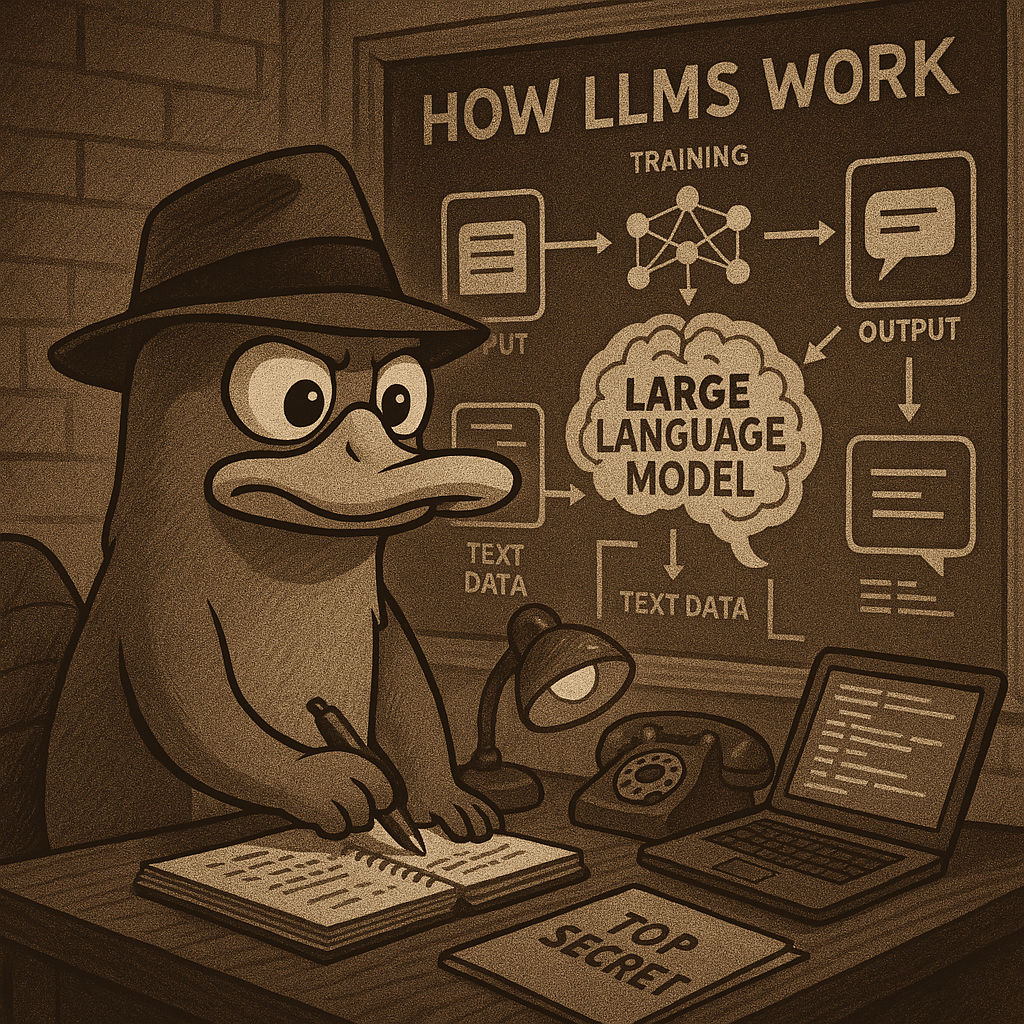
\includegraphics[width=0.6\textwidth]{agentp}
    \caption{An agent learning about LLMs}
    \label{fig:agentp}
\end{figure}
